\section{Experimento 2: Red hogareña}

\subsection{Descripción del contexto}

El experimento fue realizado en una red doméstica, por medio de una conexión Wi-Fi de Fibertel. Al momento de tomar las mediciones estaban conectados a la red una laptop, una smart TV, un celular y una tablet, entre otras cosas. La fecha de la captura fue Sábado 7 de Octubre de 2017. El celular estaba siendo usado para controlar el programa VLC por remoto.

\subsection{Descripción de la captura}

Capturamos 10000 paquetes. En la figura~\ref{protocolos2} se muestra la distribución de protocolos dentro de la captura. Observamos que hay paquetes de tipo IPv4, \texttt{0x86dd} (IPv6), ARP y también Fast Roaming Internet Request. Este último es un protocolo que permite la comunicación continua con dispositivos en movimiento. 

\begin{figure}[H]
\centering
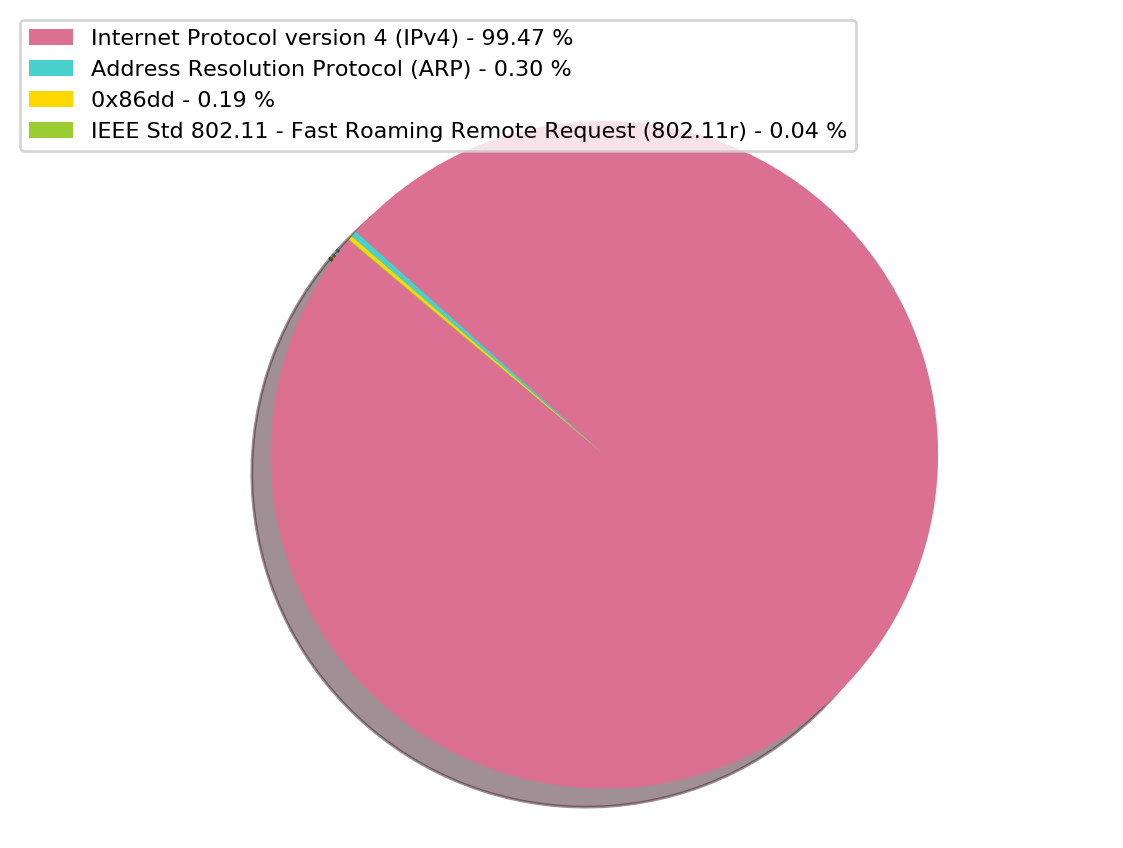
\includegraphics[width=0.7\textwidth]{protocolosRed2.png}
\caption{Gráfico que muestra la distribución de protocolos en la red.}
\label{protocolos2}
\end{figure}

En la figura~\ref{broadcast2} podemos ver el porcentaje de paquetes broadcast comparado con el total de paquetes. Vemos que esto representa un 1,8\% del total. En la figura~\ref{entropias1_2} vemos que los protocolos que aparecen en los paquetes de broadcast son ARP e IPv4. El porcentaje de broadcast es mucho menor al de la primer red porque hay menos dispositivos en uso.

\begin{figure}[H]
\centering
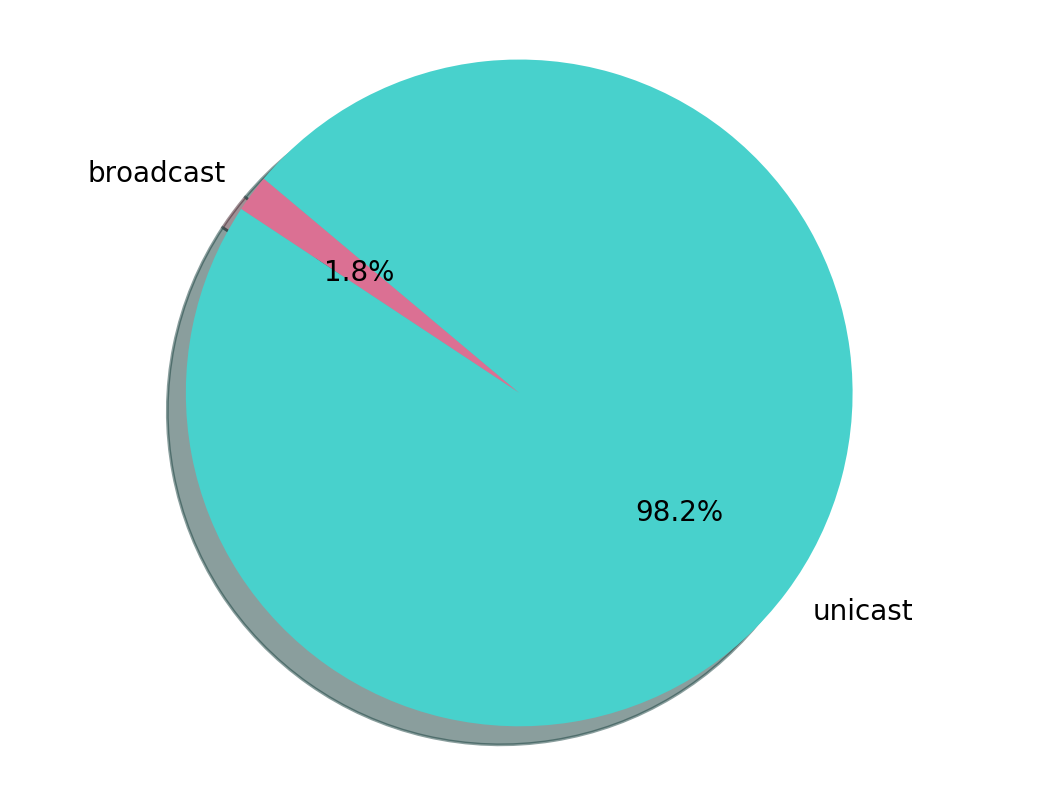
\includegraphics[width=0.7\textwidth]{broadcastRed2.png}
\caption{Gráfico que muestra los porcentajes de tráfico broadcast y unicast.}
\label{broadcast2}
\end{figure}

\subsection{Análisis de la captura}

En la figura~\ref{entropias1_2} se encuentra la información de cada símbolo de la fuente $S_1$ para esta red. Observamos que hay un símbolo cuya información es muy baja en comparación con la de los demás (IPv4, unicast); y esto hace que la entropía muestral sea mucho menor a la máxima.

\begin{figure}[H]
\centering
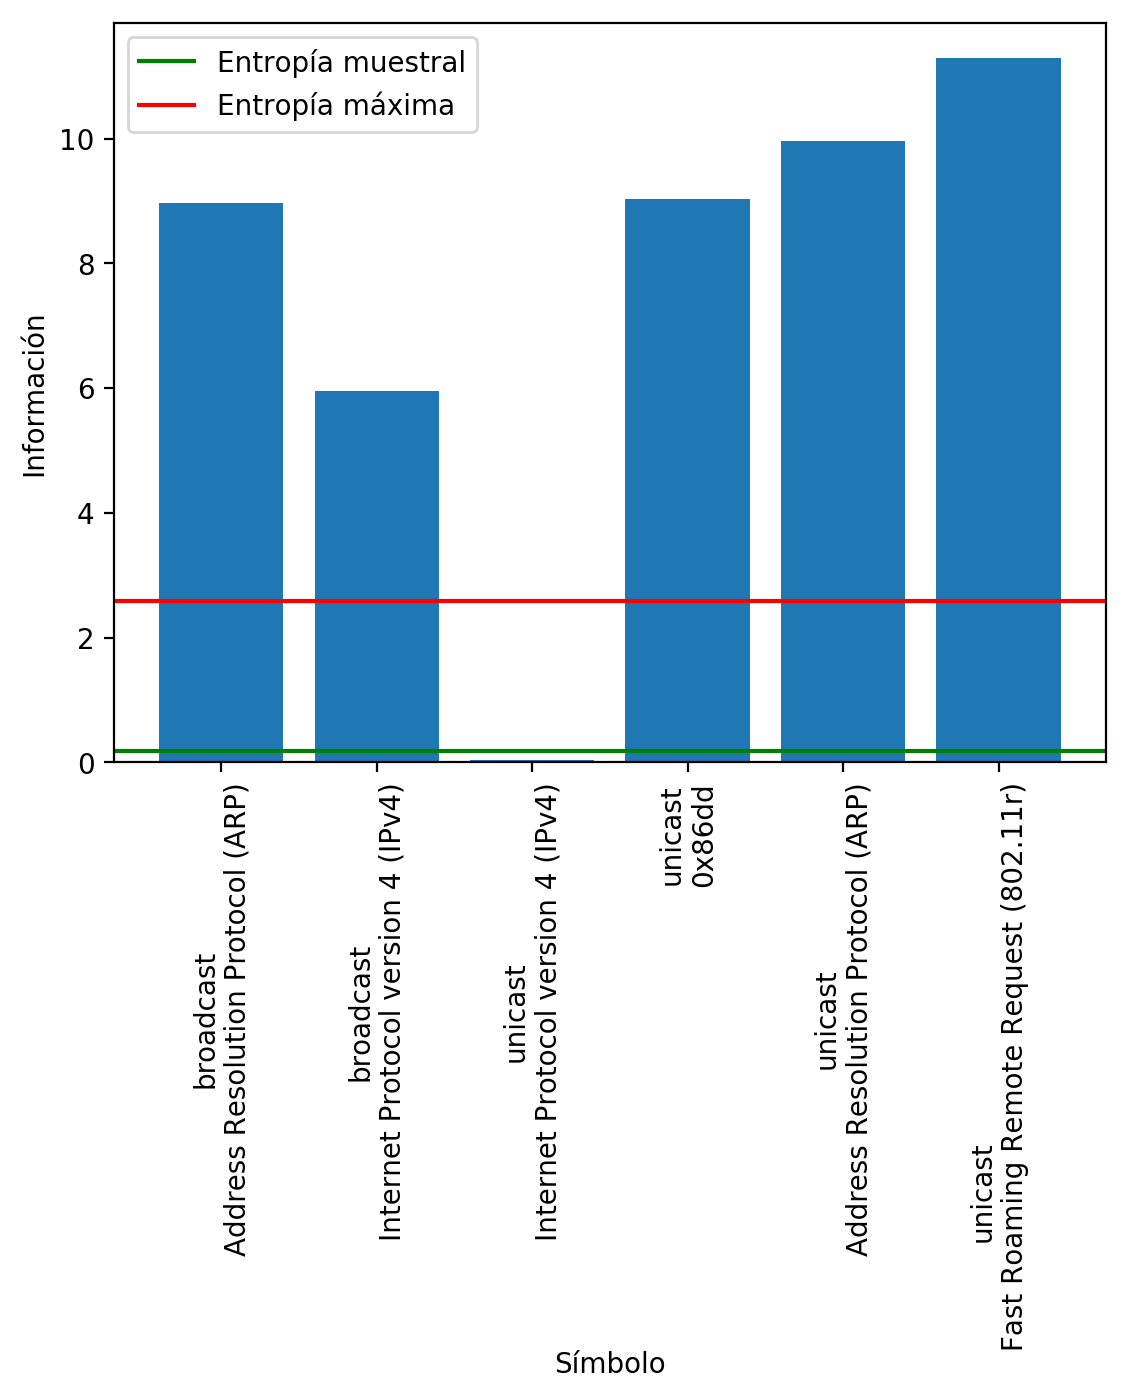
\includegraphics[width=0.7\textwidth]{entropiaS1Red2.png}
\caption{Gráfico de la información de los símbolos de la fuente $S_1$ observados en esta red. Se muestra la entropía muestral de $S_1$ y su entropía máxima.}
\label{entropias1_2}
\end{figure}

En el caso de la fuente $S_2$, como podemos ver en la figura~\ref{entropias2_2}, hay dos IPs particulares que aportan menos información que las otras, esto significa que es más común que envíen requests de ARP. En este caso, al aportar todos los símbolos aproximadamente la misma información, la entropía muestral se encuentra cerca de la máxima.

\begin{figure}[H]
\centering
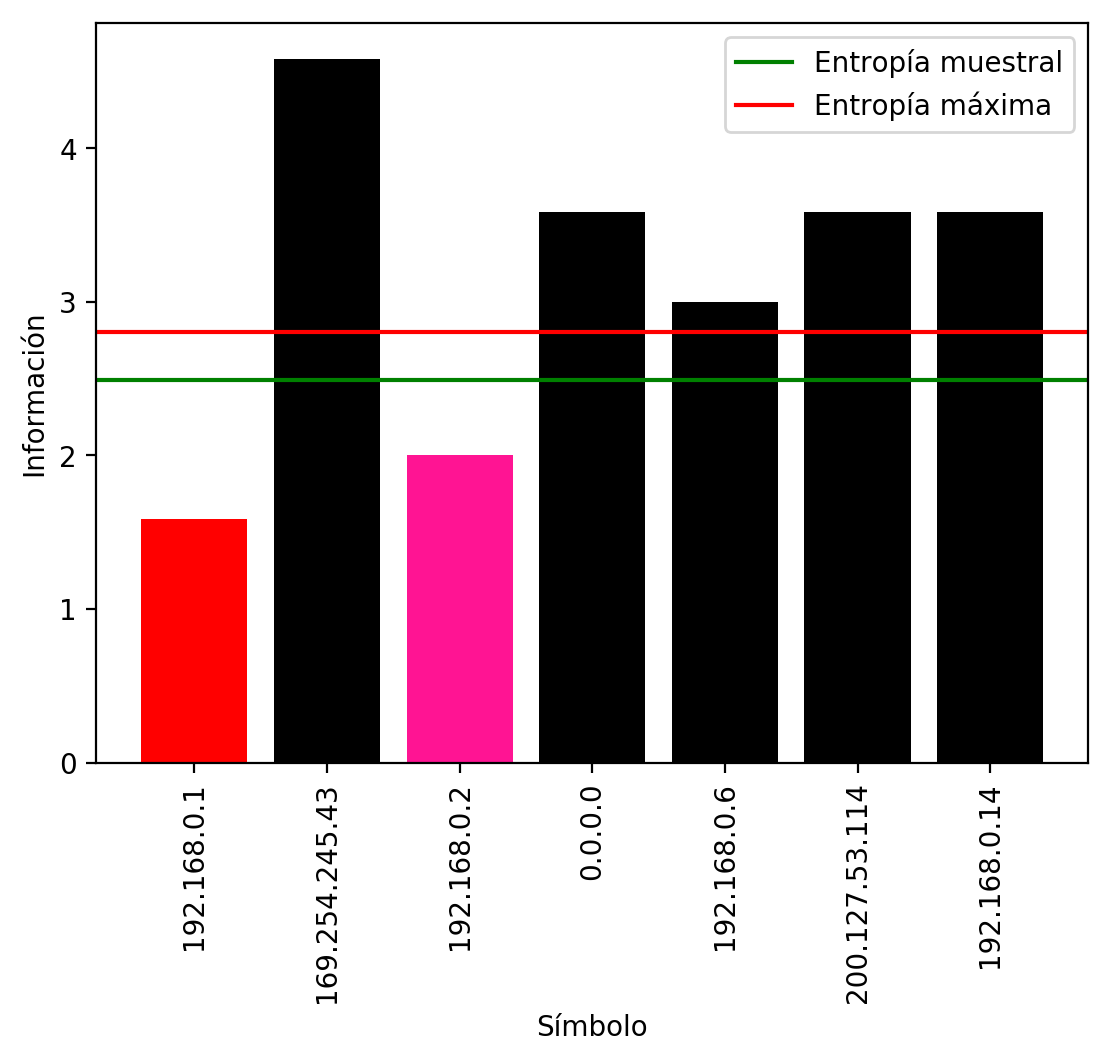
\includegraphics[width=0.7\textwidth]{entropiaS2Red2.png}
\caption{Gráfico de la información de los símbolos de la fuente $S_2$ observados en esta red. Se muestra la entropía muestral de $S_2$ y su entropía máxima.}
\label{entropias2_2}
\end{figure}

Graficamos la red subyacente de mensajes ARP en la figura~\ref{grafo2}. Los nodos representan a los hosts y las aristas los mensajes ARP de los dos tipos. No observamos ningún nodo particularmente distinguido.

\begin{figure}[H]
\centering
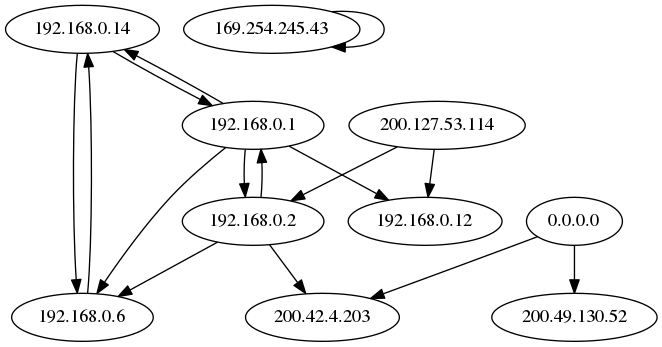
\includegraphics[width=0.7\textwidth]{grafoRed2.png}
\caption{Grafo de la red de mensajes ARP subyacente. Los nodos son las IPs observadas y los ejes son los mensajes ARP. En colores se marcan los nodos distinguidos (información por debajo de la entropía) y sus mensajes salientes. Cada arista tiene anotada la cantidad de requests/replies ARP.}
\label{grafo2}
\end{figure}
